Based on the \emph{policy-based design} \cite{a-rotm-02}, 
we represent a subdivision as a refinement function 
(\emph{host function}) parameterized with the masks
(\emph{policies}). For example, a Catmull-Clark subdivision
is structured as a primal quadralization function with the 
Catmull-Clark mask rules.
\begin{lstlisting}
void CatmullClark_subdivision(Polyhedron& p) {
  quadralize_polyhedron<CatmullClark_rule<Polyhedron>>(p);
}
\end{lstlisting}
The \lstinline!quadralize_polyhedron<>()! is the host function
refining the input mesh and maintaining the stencil 
correspondence of the PQQ scheme. The \lstinline!CatmullClark_rule!
is the policy class implementing the Catmull-Clark masks. 
Different refinement has different proper set of policies, 
i.e.\ the stencils. A PQQ scheme has facet-, edge- and vertex-stencils 
and a DQQ scheme has only corner-stencils (Figure \ref{fig:RefMap}).
In the \CC\ format, the policy class (simplified without template 
parameter) for the Catmull-Clark subdivision 
is like,
\begin{lstlisting}
class CatmullClark_rule {
public:
  void facet_rule(Facet_handle facet, Point& pt);
  void edge_rule(Halfedge_handle edge, Point& pt);
  void vertex_rule(Vertex_handle vertex, Point& pt);
};
\end{lstlisting}
The mask is a simplified mesh traversal problem as
only the attributes of the stencil need to be  
visited and collected. The stencil has a 1-ring 
neighnorhood of a vertex, a edge or a facet.
To implement a facet setncil of the 
Catmull-Clark subdivision, we circulate around 
the facet vertices and aplly the mask.
\begin{lstlisting}
void facet_rule(Facet_handle facet, Point& pt) {
  Halfedge_around_facet_circulator hcir = facet->facet_begin();
  Vector vec = hcir->vertex()->point() - CGAL::ORIGIN;
  ++hcir;
  do {
    vec = vec + hcir->vertex()->point();
  } while (++hcir != facet->facet_begin());
  pt = CGAL::ORIGIN + vec/circulator_size(hcir);
}
\end{lstlisting}
The \lstinline!Facet_handle facet! points to the stencil
source and the \lstinline!Point& pt! specifies the
target vertex. For this specific mask, we compute the
centroid with a loop based on a circulator over the halfedges
surrounding a facet. The CGAL kernel geometry, i.e. Points 
and Vectors computation, is used. Though for a specialized
kernel, special computation may be applied in user-defined
policies.
 
Implementating a topology refinement is a rather complex job.  One
approach is to encode the refinement into a sequence of Euler
operations. For Catmull-Clark subdivision, the refinement is encoded
as edge-vertex insertions, edge insertion between two neighboring
edge-vertices, facet-vertex insertion on he inerted edge, and then
edge insertions between the facet-vertex the edge-vertices. 
The sequence is demonstrated in Figure \ref{fig:CCRefinement}. 
Note that the vertex and edge insertions can be easily 
implemented based on the Euler operations supported by \cgalpoly.
\begin{figure}
  \centering
  \epsfig{file=figs/CCRefinement.eps, width=7cm}
  \caption{A PQQ refinement of a facet is encoded into a sequence of
  vertex insertions and edge insertions. Red indicates the inserted
  vertices and edges on each step.}
  \label{fig:CCRefinement}
\end{figure}

The stencil correspondence of the refinement is assured
by the the traversal sequence of the mesh. The host function
has a two pass algorithm. The first pass generates the
points by calling the polcies. The second pass
refines the mesh with a sequence of the Euler operations.
The points generated in the first pass are stored in a
point buffer in the order of the stencil 
travesal. The sequence of the vertex insertions 
matches the storage order of the point buffer. It assures 
the stencil correspondence of the refinement.

Most primal refinement schemes can be translated into a sequence of
Euler operations. Though dual schemes, e.g.\ Doo-Sabin subdivision,
have no simple translation of Euler operations. A sequence
of Euler operations for a DQQ scheme consists of two times 
of the midedge refinement \ref{Peters:1997:SSS} and 
result an inefficient implementation.
To support such schemes efficiently, we use the modifier 
callback mechanism of \cgalpoly\ to rebuild the mesh
connectivity. In addition to the points buffer, we
also create a facet list based on the source mesh. Note that in a DQQ
scheme, every new facet corresponds to a vertex, edge or facet. The
combination of the points buffer and facet list represents a
facet-vertex index list which indexes the vertices and enumerates each
facet as an index sequence. A modifier creating a polyhedron from a
facet-vertex index list is then a simple task.
\begin{lstlisting}
pb.begin_surface(num_point, num_facet); {
  for (int i = 0; i < num_point; ++i) 
    pb.add_vertex(Point(point_buffer[i*3+0], 
	          point_buffer[i*3+1], 
	          point_buffer[i*3+2]));	
  for (int i = 0; i < num_facet; ++i) {
    pb.begin_facet(); {
      for (int n = 0; n < facet_buffer[i][0]; ++n)
      pb.add_vertex_to_facet(facet_buffer[i][n+1]);
    }
    pb.end_facet();
  }
}
pb.end_surface();
\end{lstlisting}

Our subdivision solution, decoupling the geometry rules from the
refinement, grants users the flexible control of the mask.
Variants of the subdivisions can be devised by simply replacing
the policies. As the solution is not restricted by the 
mesh configurations (in contrast to the quad-tree or patch-based 
implementation), subdivision pipeline is easily supported
as a composite funtion like
\begin{lstlisting}
void MySubdivision(Polyhedron& p) {
  quadralize_polyhedron<Myrule_1<Polyhedron>>(p);
  dualize_polyhedron<Myrule_2<Polyhedron>>(p);
} 
\end{lstlisting}

More importantly, our solution accepts a user-specialized 
polyhedron. No special flag or attribute is required 
to assist the \tr . This generality make our solution natually fit 
in a modeling pipeline or a multipass modeling enviroment. 

%TODO: since the writing memory is not overlapped, multi-threaded
%supporting is easily done.

%TODO: trade-off between generic and efficient.
 
